\section{Блоки Pioneer Bricks: программа без кода}
\label{sec:bricks}

\begin{infobox}[Цели главы]
\begin{itemize}
    \item Понимать, что такое Pioneer Bricks и где запускается блочная программа.
    \item Собирать программы для Пионера Мини~2 из блоков: светодиоды, датчики, полёт, камера, нейросети.
    \item Читать код, который Bricks генерирует из блоков, и связывать блоки с вызовами \texttt{pioneer\_sdk2} и \texttt{pioneer\_rknn}.
    \item Знать ограничения версии Bricks~2.3.0 и уметь их обходить.
\end{itemize}
\end{infobox}

\begin{missionbox}[Блоки в симуляторе]
В симуляторе у Пионера Мини~2 доступен набор блоков по образцу Bricks (редактор $\to$ \ui{Мини 2} $\to$ язык Blockly). Часть блоков с камерой и нейросетями в симуляторе упрощена или доступна только на дроне, поэтому программы этой главы целиком запускаются на борту, а в симуляторе удобно отрабатывать полётные блоки и логику.
\end{missionbox}

\subsection{Что такое Pioneer Bricks}

Предыдущие главы были про текстовые программы на Python, которые работают на самом дроне. Но программировать можно и без текста. \textbf{Pioneer Bricks} --- официальная среда визуального программирования Геоскана, построенная на Google Blockly. Программа собирается из цветных блоков, как пазл: блок «Взлёт» нельзя вставить туда, где нужно число, а блок с числом --- туда, где нужна команда. Синтаксических ошибок, которые мучают новичка в тексте (забытая скобка, неверный отступ), в блоках просто не бывает.

Главное для нас: Bricks не изобретает свой язык. При сохранении он \emph{генерирует программу на Python}, которая использует те же библиотеки \texttt{pioneer\_sdk2} и \texttt{pioneer\_rknn}, что и главы~\ref{sec:sdk2} и~\ref{sec:rknn}. Поэтому Bricks --- удобная ступень перед текстом: любой блок можно «раскрыть» и увидеть, какой вызов за ним стоит. Глава написана по версии \textbf{Bricks 2.3.0}; все десять проектов проверены на Пионере Мини~2 (Pioneer~OS 1.0.0, \texttt{pioneer\_sdk2} 0.16.0, \texttt{pioneer\_rknn} 1.10.0).

\paragraph{Где это запускается.} Bricks работает на борту Мини~2, как и среда Pioneer Code. Подключитесь к Wi-Fi дрона и откройте в браузере главное меню Pioneer Code (\texttt{http://10.42.0.1:9090}), в нём пункт «Pioneer Bricks», либо сразу \texttt{http://10.42.0.1:2020}. Программа выполняется на дроне, а не в браузере.

\begin{alertbox}[Кнопка «Вжух» запускает программу на дроне]
Кнопка \ui{Вжух} в правом верхнем углу редактора \emph{выполняет} программу на дроне. Если в ней есть блоки из категории «Полёт» (\emph{Предполётная подготовка}, \emph{Взлёт}, \emph{Лететь в…}), дрон запустит двигатели и взлетит. Перед нажатием проверьте программу, площадку и людей вокруг; кнопка \ui{Стоп} рядом прерывает выполнение. Правила безопасности те же, что в главе~\ref{sec:sdk2}: пульт в руках, свободная площадка, аварийная остановка под рукой.
\end{alertbox}

Из десяти проектов главы полётный только пятый, он помечен отдельно. Остальные выполняются при выключенных двигателях: дрон стоит на земле. Пока блоки категории «Полёт» не нужны, не добавляйте их в программу.

\subsection{Проекты и редактор}

\begin{figure}[H]
\centering
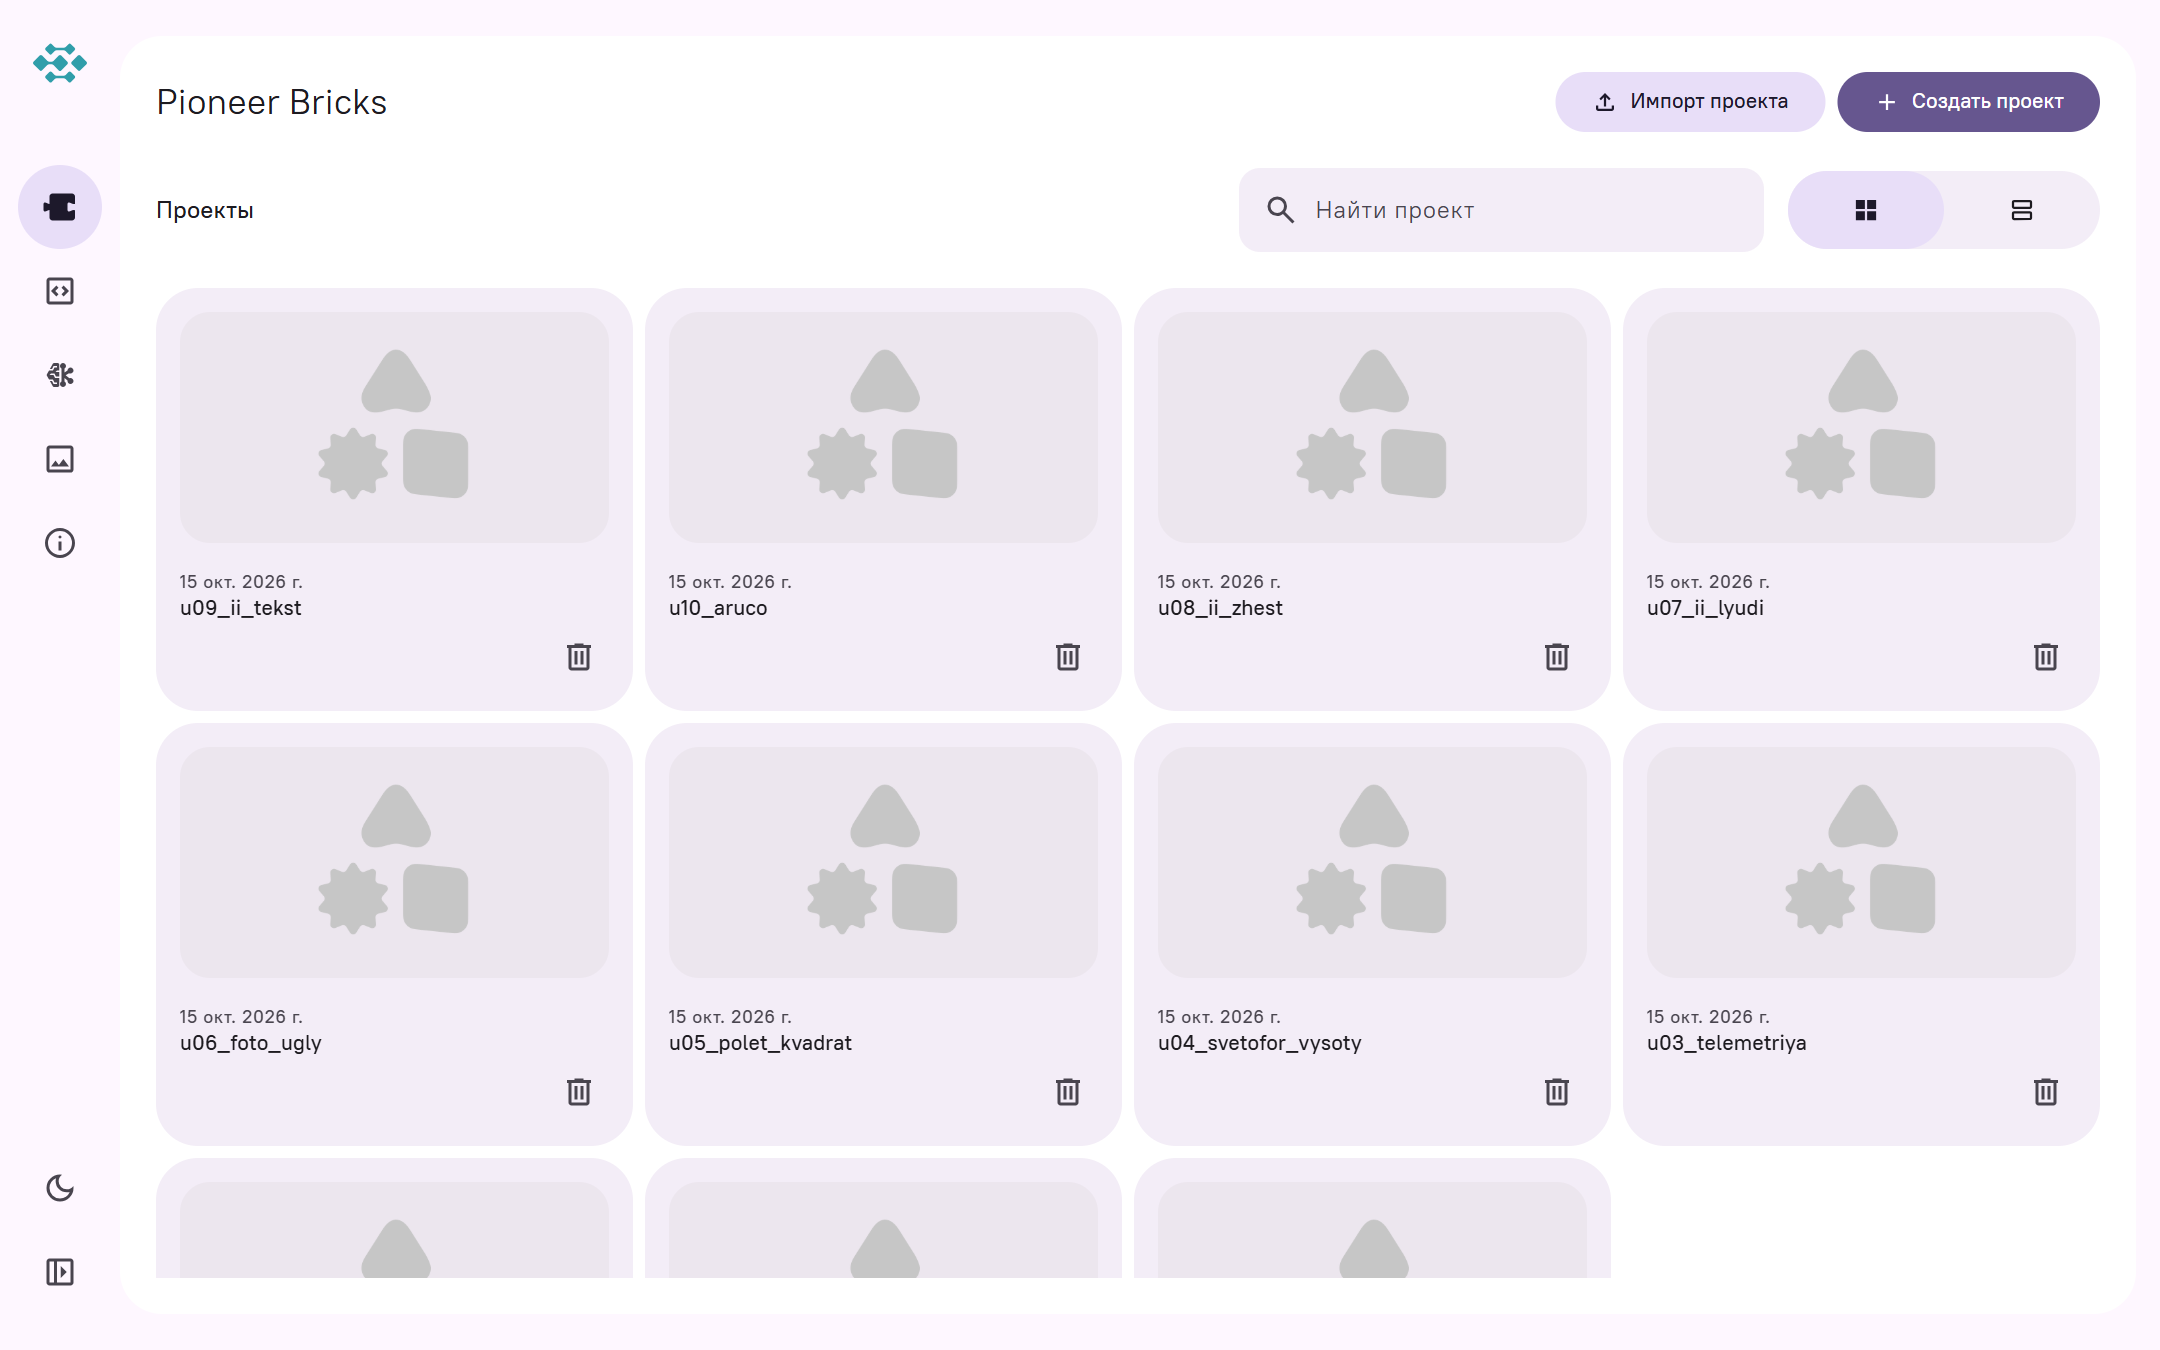
\includegraphics[width=\textwidth]{images/bricks/b00_projects.png}
\caption{Стартовая страница Bricks: «Создать проект», «Импорт проекта» и список проектов на дроне}\label{fig:bricks-projects}
\end{figure}

Проекты хранятся на дроне в папке \texttt{/usr/local/bin/pioneer-bricks/static/save/<имя>/}: файл \texttt{<имя>.xml} --- блоки, \texttt{<имя>.py} --- сгенерированный Python (появляется после сохранения). Кнопки «скачать» и «загрузить» в редакторе экспортируют и импортируют проект целиком, так проекты переносят между дронами. К главе приложены десять готовых проектов --- файлы \texttt{.xml} в папке \texttt{examples/python-onboard/bricks/}: нажмите «Импорт проекта» и выберите файл.

\begin{figure}[H]
\centering
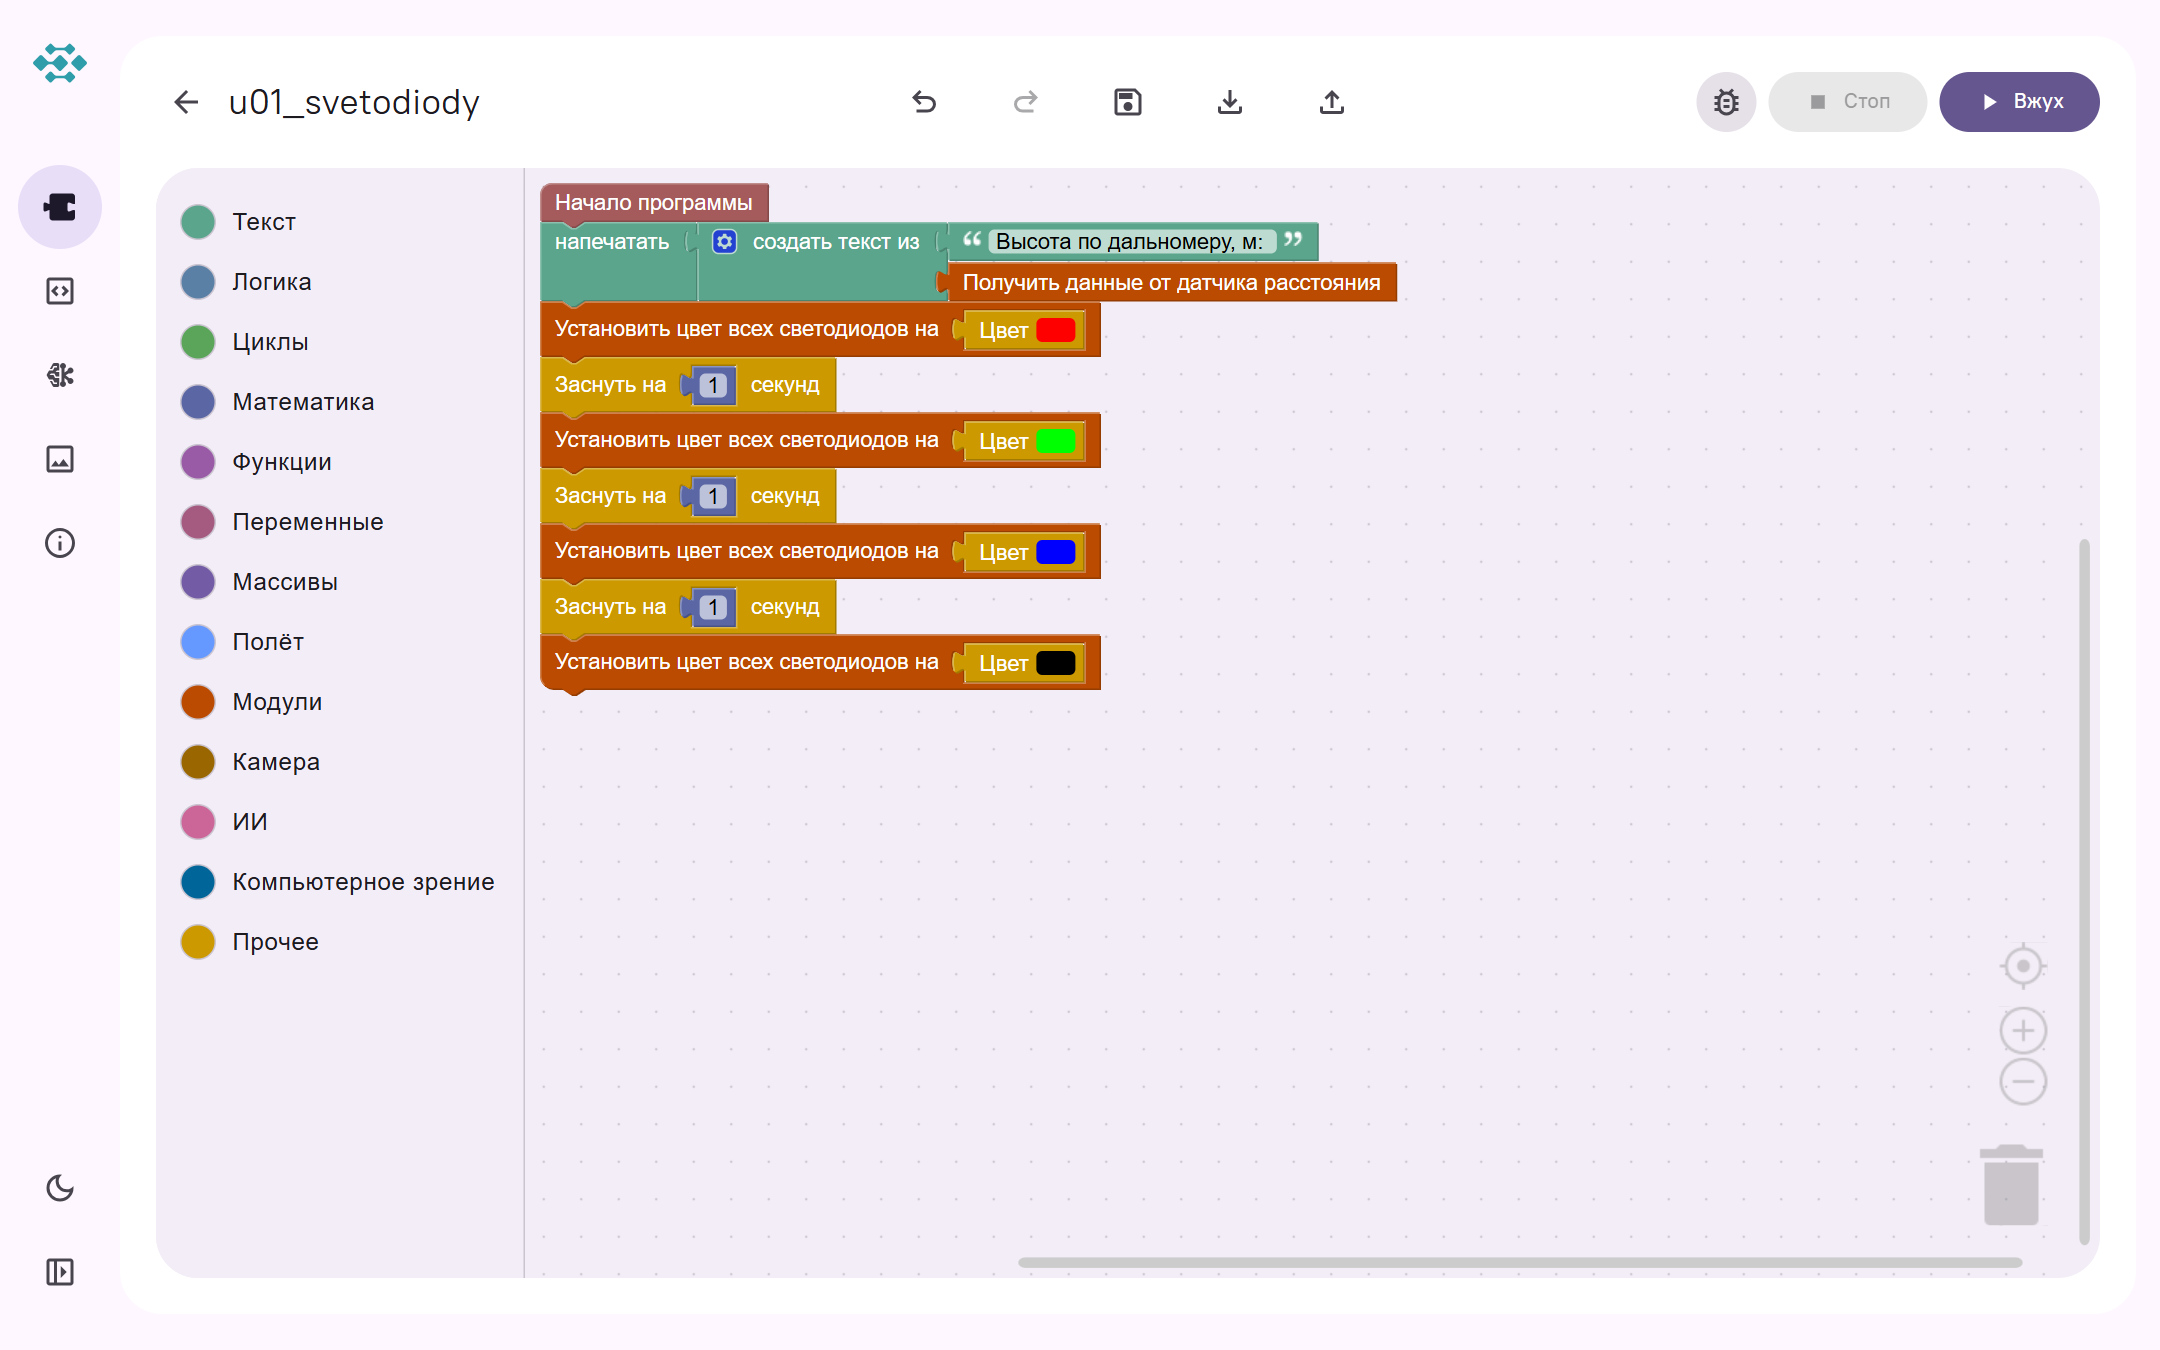
\includegraphics[width=\textwidth]{images/bricks/u01_svetodiody.png}
\caption{Редактор Bricks с проектом первого задания}\label{fig:bricks-editor}
\end{figure}

\begin{center}\small
\begin{tabularx}{\linewidth}{@{}>{\raggedright\arraybackslash}p{0.3\linewidth}X@{}}
\toprule
\textbf{Элемент} & \textbf{Назначение} \\
\midrule
Палитра слева & категории блоков; щелчок открывает список, блок перетаскивается на рабочее поле \\
Рабочее поле & программа; выполнение начинается с неудаляемого блока «Начало программы» и идёт сверху вниз \\
Изогнутые стрелки & отменить / повторить действие \\
Дискета & «Сохранить» / «Сохранить как»: сохраняет блоки \emph{и} генерирует Python \\
Стрелки вниз / вверх & экспорт проекта в файл / импорт \\
Жук & режим отладки \\
\ui{Стоп} / \ui{Вжух} & остановить / \textbf{запустить программу на дроне} \\
Справа внизу & центрирование, масштаб, корзина (перетащите блок в неё, чтобы удалить) \\
\bottomrule
\end{tabularx}
\end{center}

При запуске под полем появляются панели «Вывод программы» (то, что печатают блоки «напечатать») и «Просмотр изображений» (окна, в которые программа отправляет кадры блоком «Демонстрация изображения»). Те же окна открываются в браузере по адресу \texttt{http://10.42.0.1:8889/<имя окна>/}, как у \verb|ImageViewer| в главе~\ref{sec:sdk2}.

\subsection{Блоки по категориям}

\begin{center}\small
\begin{tabularx}{\linewidth}{@{}>{\raggedright\arraybackslash}p{0.27\linewidth}X@{}}
\toprule
\textbf{Категория} & \textbf{Что внутри} \\
\midrule
Текст, Логика, Циклы, Математика & стандартные блоки Blockly: строки и печать, «если / иначе», сравнения, повторения, арифметика --- то же, что в главах про основы Python \\
Функции, Переменные, Массивы & свои функции, переменные (\emph{присвоить}, \emph{получить}), списки \\
\textbf{Полёт} & предполётная подготовка (запуск двигателей), взлёт, посадка, полёт в точку, ожидание точки, скорости, курс \\
\textbf{Модули} & сервопривод камеры, захват, Ranger, светодиоды, дальномер, ориентация, координаты и скорости \\
\textbf{Камера} & получить кадр, показать в окне, сохранить фото, размер, поворот, отражение, обрезка, рисование \\
\textbf{ИИ} & модель (Yolo, YoloPose, PaddleOCR), поиск объектов и поз, распознавание текста \\
\textbf{Компьютерное зрение} & маркеры ArUco, координаты и размер объекта, размытие, Кэнни, цветовые и бинарные маски, контуры \\
Прочее & пауза «Заснуть на», время, выбор цвета, угла, точки \\
\bottomrule
\end{tabularx}
\end{center}

Содержимое палитр, специфичных для дрона, показано на рис.~\ref{fig:bricks-palettes} и~\ref{fig:bricks-palettes2}.

\begin{figure}[p]
\centering
\begin{minipage}[t]{0.49\textwidth}\centering
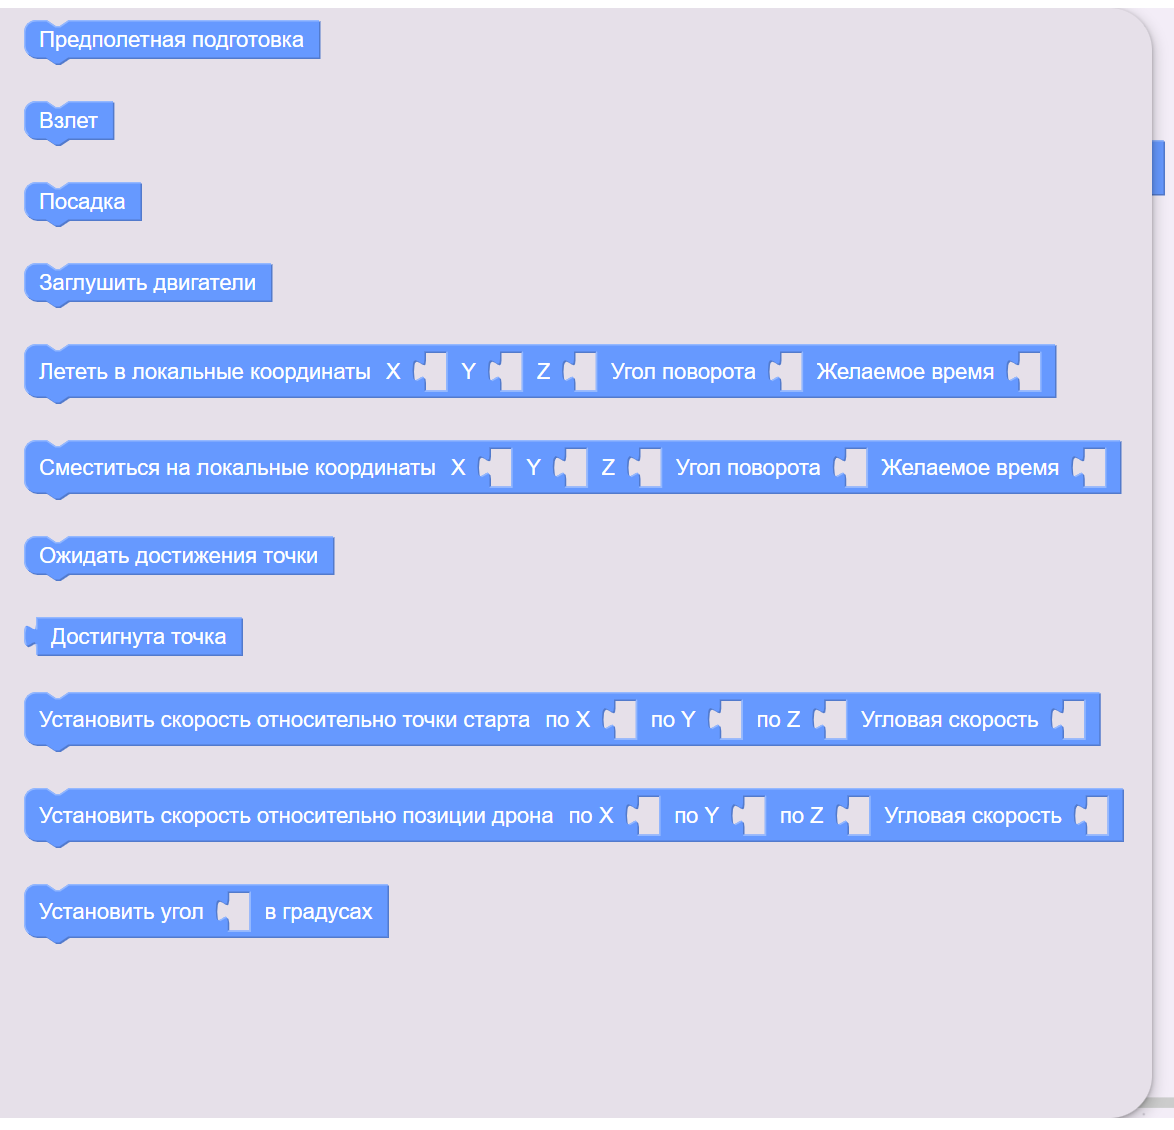
\includegraphics[width=\linewidth]{images/bricks/cat_08.png}
\par\smallskip{\sffamily\small Полёт}
\end{minipage}\hfill
\begin{minipage}[t]{0.49\textwidth}\centering
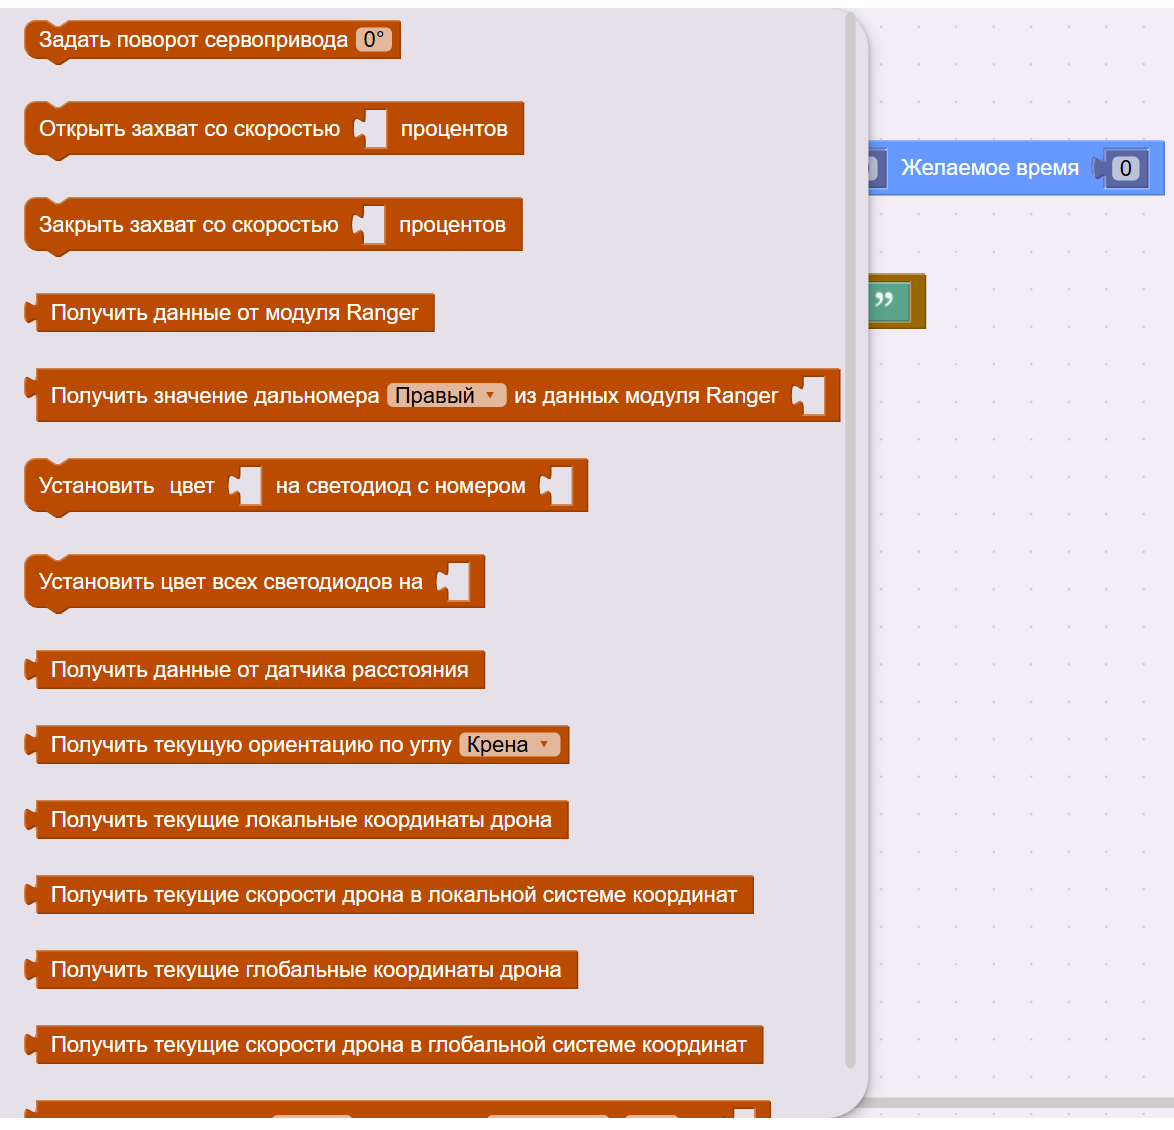
\includegraphics[width=\linewidth]{images/bricks/cat_09.png}
\par\smallskip{\sffamily\small Модули}
\end{minipage}

\medskip
\begin{minipage}[t]{0.49\textwidth}\centering
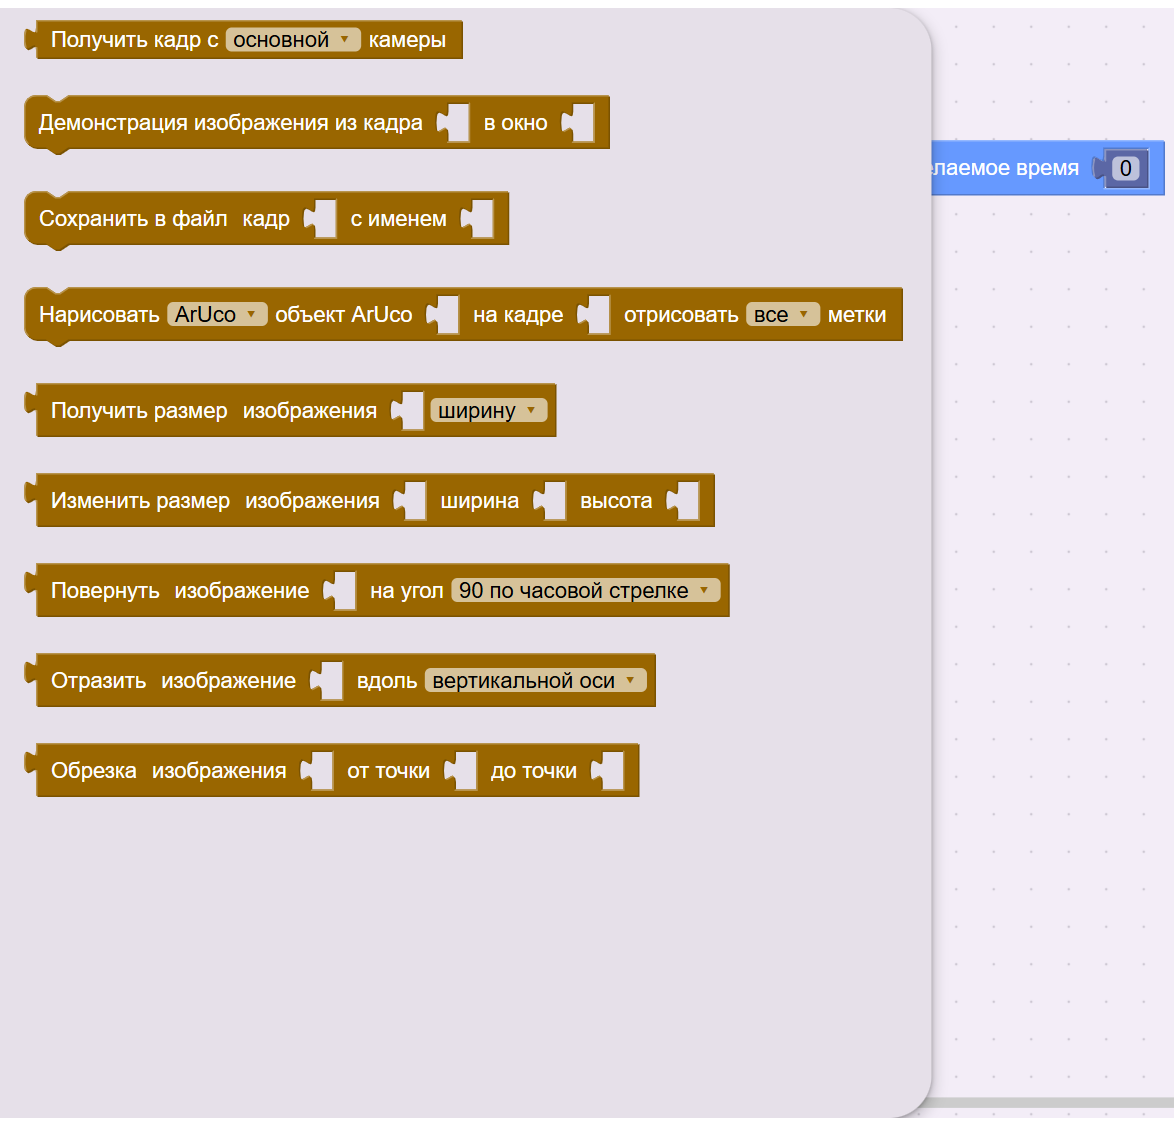
\includegraphics[width=\linewidth]{images/bricks/cat_10.png}
\par\smallskip{\sffamily\small Камера}
\end{minipage}\hfill
\begin{minipage}[t]{0.49\textwidth}\centering
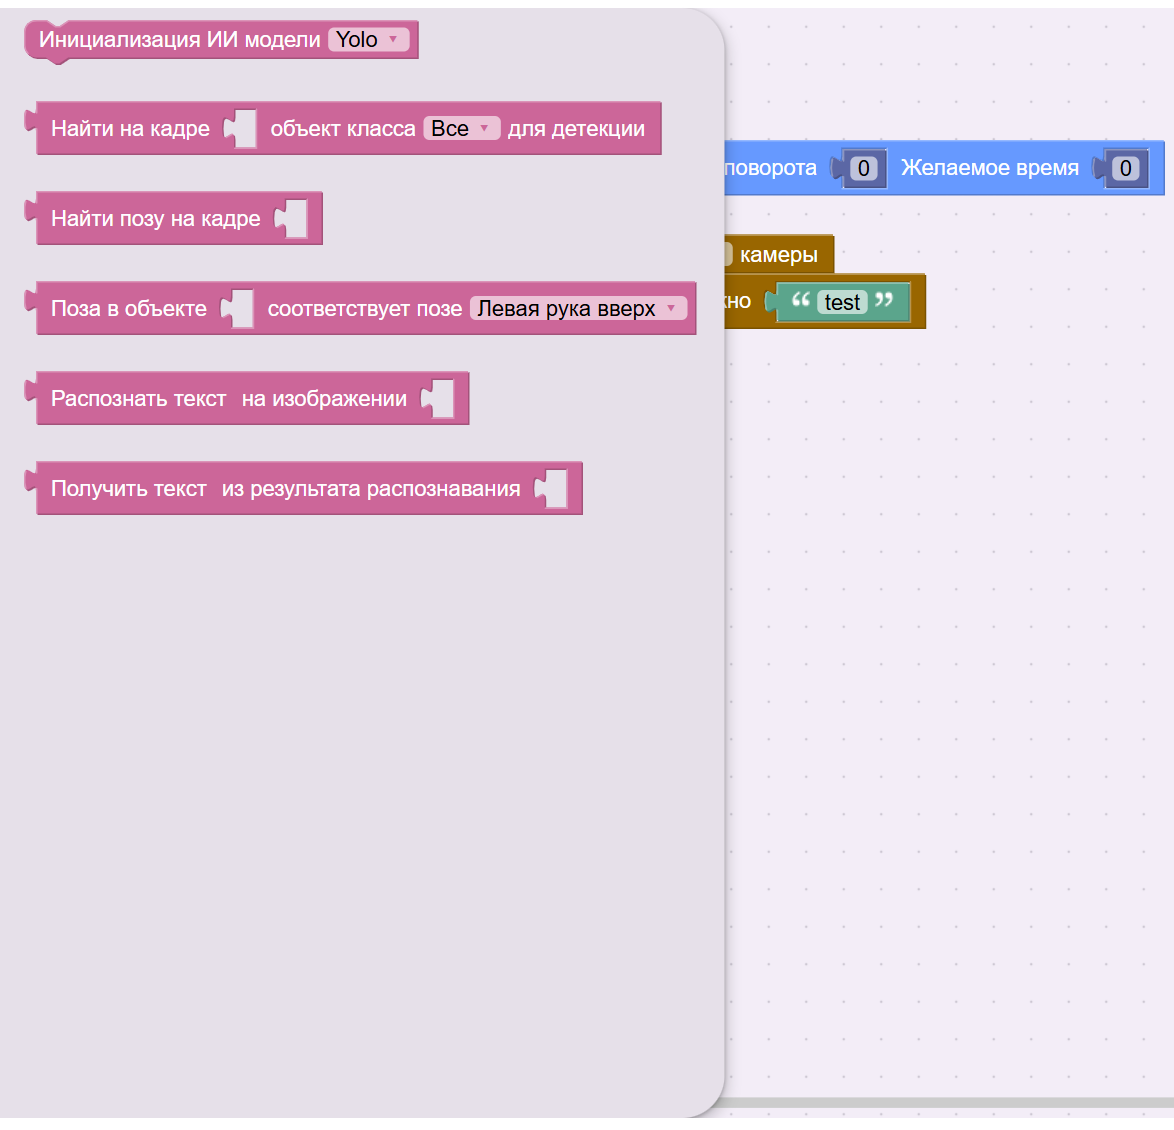
\includegraphics[width=\linewidth]{images/bricks/cat_11.png}
\par\smallskip{\sffamily\small ИИ}
\end{minipage}
\caption{Палитры блоков для дрона}\label{fig:bricks-palettes}
\end{figure}

\begin{figure}[H]
\centering
\begin{minipage}[t]{0.32\textwidth}\centering
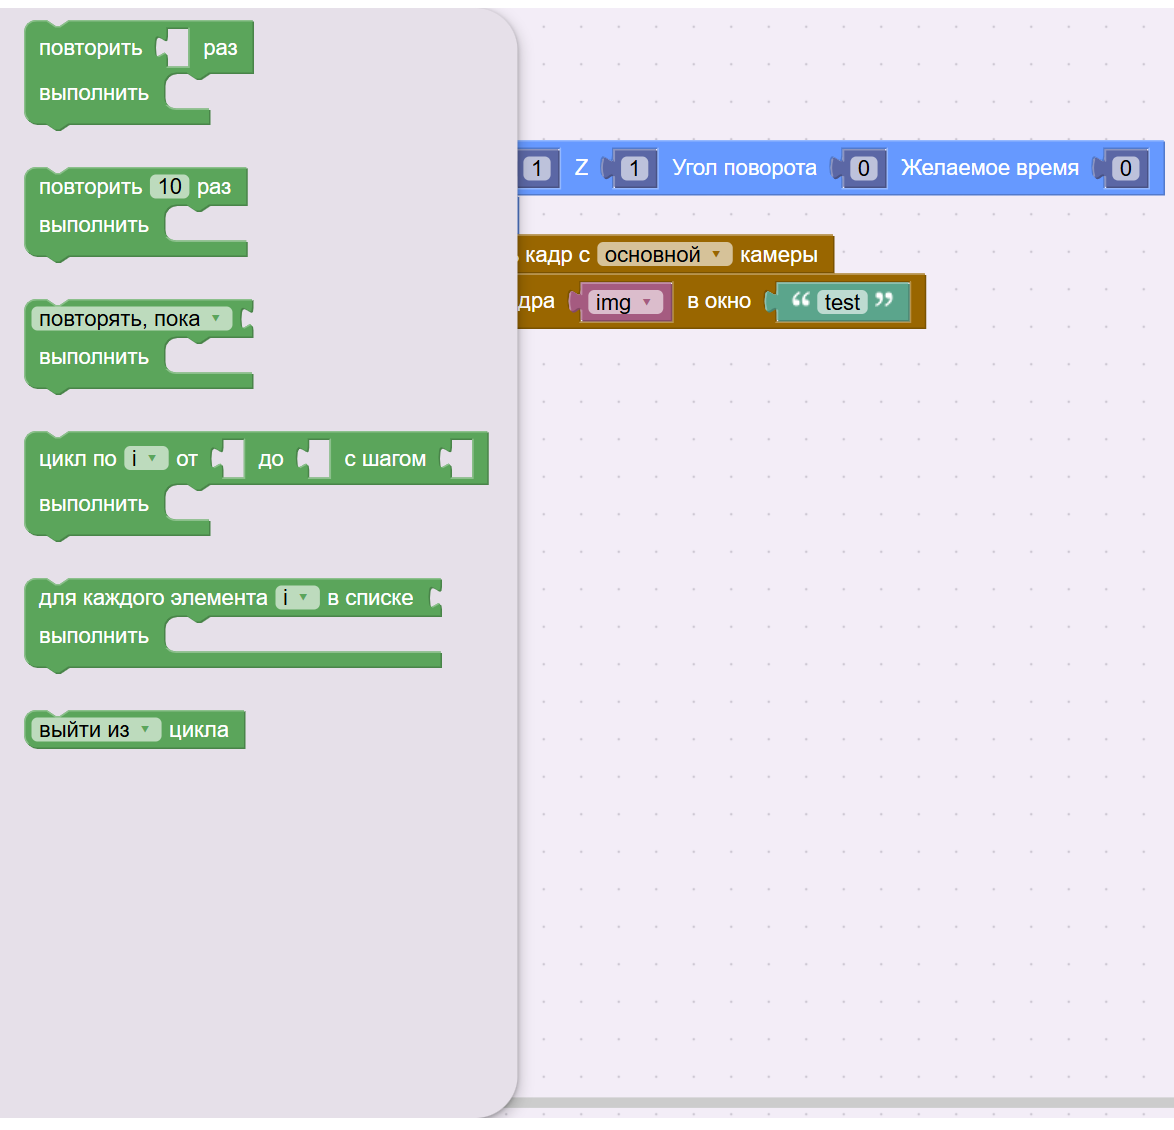
\includegraphics[width=\linewidth]{images/bricks/cat_03.png}
\par\smallskip{\sffamily\small Циклы}
\end{minipage}\hfill
\begin{minipage}[t]{0.32\textwidth}\centering
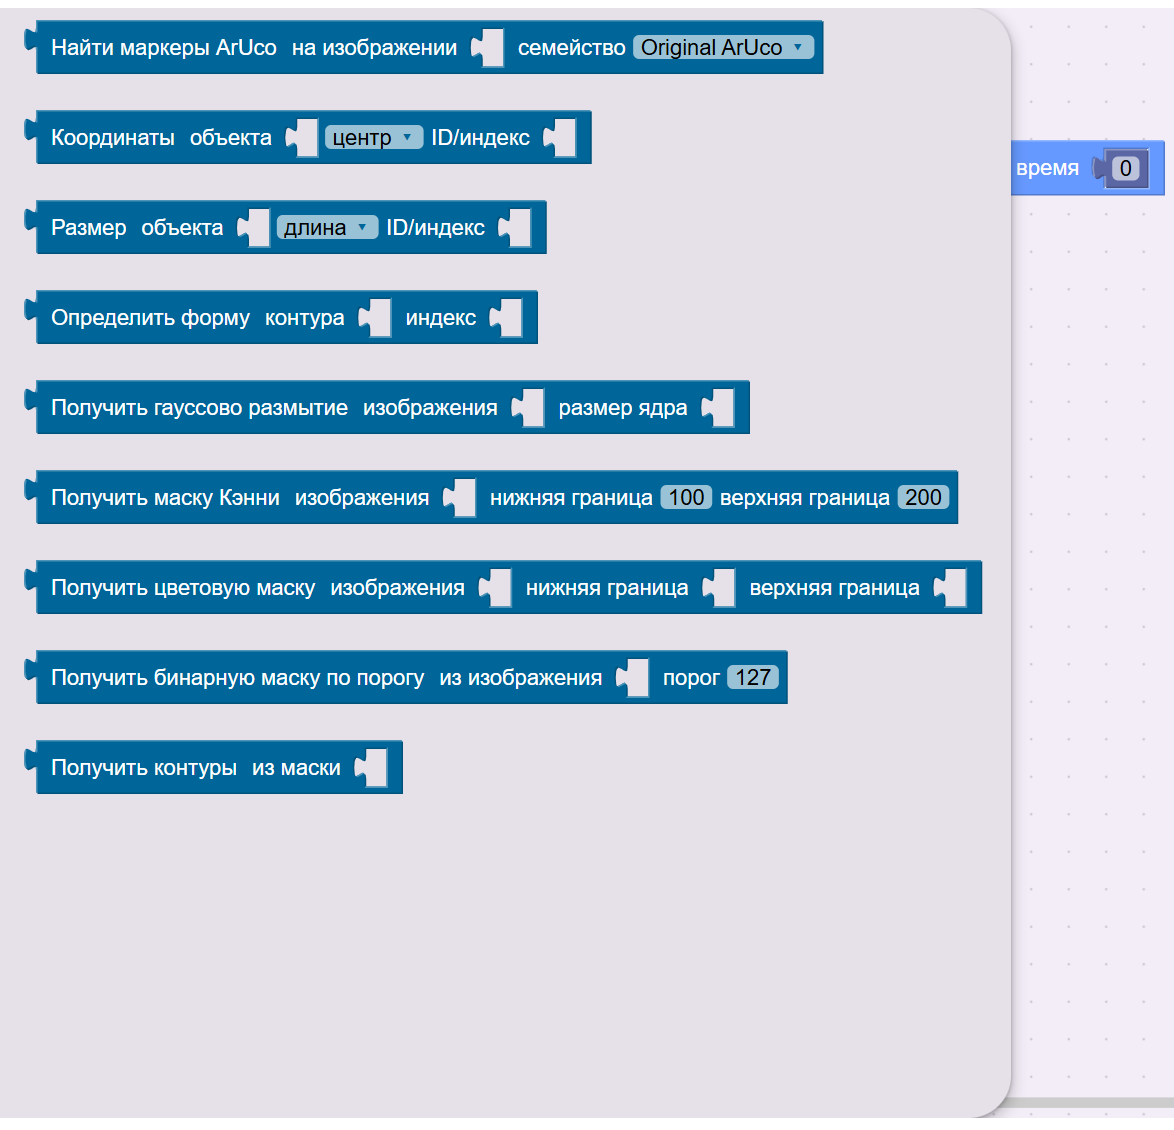
\includegraphics[width=\linewidth]{images/bricks/cat_12.png}
\par\smallskip{\sffamily\small Компьютерное зрение}
\end{minipage}\hfill
\begin{minipage}[t]{0.32\textwidth}\centering
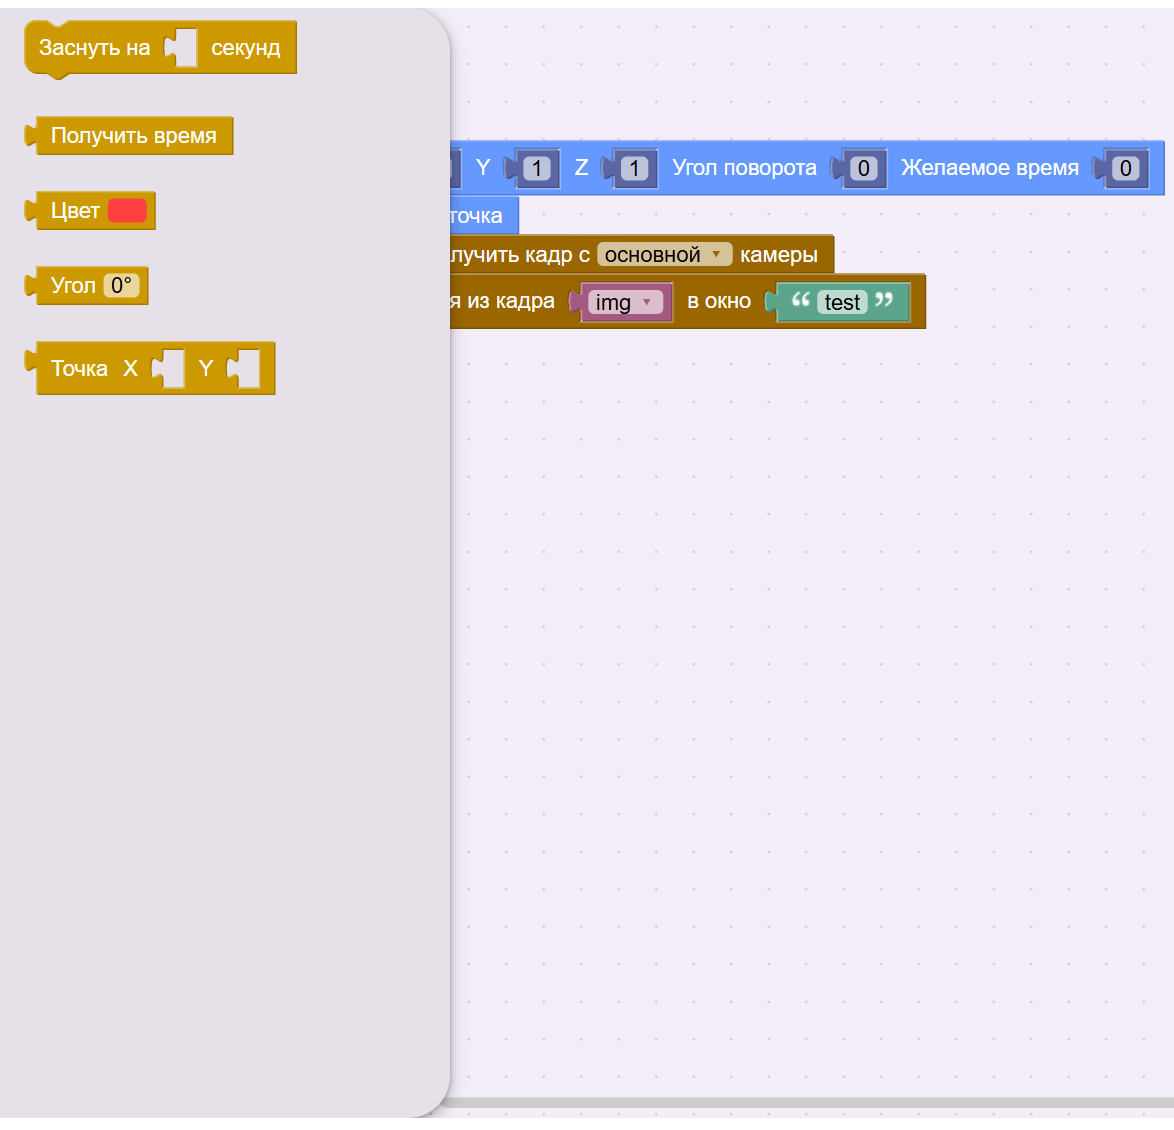
\includegraphics[width=\linewidth]{images/bricks/cat_13.png}
\par\smallskip{\sffamily\small Прочее}
\end{minipage}
\caption{Ещё три палитры}\label{fig:bricks-palettes2}
\end{figure}

\subsection{Во что превращаются блоки}

Сгенерированный файл всегда устроен одинаково: импорты и создание объектов (\verb|Pioneer()|, камеры, \verb|ImageViewer|, модели), затем \emph{тело программы} внутри \verb|try|, а в \verb|finally| --- безопасное завершение. Вот полный файл самой короткой программы (проект~3 ниже). Это та же схема «подключение $\to$ \verb|try| $\to$ \verb|finally|», что вы писали руками в главе~\ref{sec:sdk2}:

\begin{codefile}[python]{python-onboard/bricks/python/full_u03_telemetriya.py}
\end{codefile}

В остальных листингах главы показано только тело программы; оно вставляется внутрь \verb|try|. Таблица соответствия основных блоков:

\begin{center}\small
\begin{tabularx}{\linewidth}{@{}>{\raggedright\arraybackslash}p{0.36\linewidth}X@{}}
\toprule
\textbf{Блок} & \textbf{Python (\texttt{pioneer\_sdk2} / \texttt{pioneer\_rknn})} \\
\midrule
Предполётная подготовка / Взлёт / Посадка & \verb|pioneer.arm()| / \verb|pioneer.takeoff()| / \verb|pioneer.land()| \\
Лететь в локальные координаты & \verb|pioneer.go_to_local_point(x, y, z, yaw, time)| \\
Ожидать достижения точки & \verb|while not pioneer.point_reached(): pass| \\
Установить цвет всех светодиодов & \verb|pioneer.led_control(255, r, g, b)|; цвет из вида \texttt{\#RRGGBB} переводится в доли 0..1 \\
Установить цвет светодиода с номером & \verb|pioneer.led_control(i, r, g, b)| \\
Получить данные от датчика расстояния & \verb|pioneer.get_dist_sensor_data()| \\
Задать поворот сервопривода & \verb|servo.set_angle(angle=...)| \\
Получить кадр с основной камеры & \verb|cam_main.get_cv_frame()| \\
Демонстрация изображения в окно & \verb|iv.imshow(name=..., frame=...)|, окно \texttt{:8889/<имя>/} \\
Сохранить в файл кадр & \verb|cv2.imwrite(путь, кадр)|, путь \texttt{/mnt/media/photos/<имя>.jpg} \\
Инициализация ИИ модели Yolo & \verb|Yolo(model_name="yolov8n")| \\
Заснуть на & \verb|sleep(секунды)| \\
\bottomrule
\end{tabularx}
\end{center}

\begin{hintbox}[Смотрите на сгенерированный код]
Если программа из блоков ведёт себя неожиданно, откройте её \texttt{.py}-файл (в среде Pioneer Code, папка проекта Bricks): по коду почти всегда видно, в чём дело. А когда блоков станет тесно, переходите к программам на Python из глав~\ref{sec:sdk2} и~\ref{sec:rknn}: те же задачи решаются там короче и гибче.
\end{hintbox}

\subsection{Безопасное завершение}

В \verb|finally| каждой программы, которая использует \verb|pioneer|, Bricks вызывает \verb|pioneer.land()|, останавливает камеры и закрывает окна просмотра. Что бы ни случилось внутри (ошибка в блоке, нажатие \ui{Стоп}, пропавший кадр), дрон в конце садится. Это защита от «зависшего» в воздухе дрона --- то самое правило «посадка в \verb|finally|», которое в главе~\ref{sec:sdk2} вы соблюдали вручную. Здесь оно встроено, но рассчитывать только на него не нужно: полётную программу всё равно заканчивайте явным блоком «Посадка», а пульт держите в руках.

\subsection{Десять проектов}

Проекты идут по возрастанию сложности: сначала последовательность команд и циклы, затем условия и датчики, потом полёт и камера, в конце нейросети и компьютерное зрение. У каждого есть снимок блоков, сгенерированный Python (тело программы, без импортов и \verb|finally|), разбор и результат. Готовые проекты лежат в \texttt{examples/python-onboard/bricks/}. Если не сказано иное, проект выполняется на земле, при выключенных двигателях.

\begin{center}\small
\begin{tabularx}{\linewidth}{@{}c>{\raggedright\arraybackslash}p{0.32\linewidth}>{\raggedright\arraybackslash}p{0.2\linewidth}X@{}}
\toprule
\textbf{№} & \textbf{Проект} & \textbf{Файл} & \textbf{Тема} \\
\midrule
1 & Светодиоды & \texttt{u01} & последовательность команд \\
2 & Бегущий огонь & \texttt{u02} & циклы, переменная-счётчик \\
3 & Телеметрия & \texttt{u03} & датчик и вывод данных \\
4 & Светофор высоты & \texttt{u04} & условия, бесконечный цикл \\
5 & Полёт по квадрату & \texttt{u05} & полётное задание (\textbf{полёт}) \\
6 & Фото под углами & \texttt{u06} & сервопривод, кадр, файл \\
7 & ИИ: люди & \texttt{u07} & детекция Yolo \\
8 & ИИ: жест & \texttt{u08} & поза YoloPose \\
9 & ИИ: текст & \texttt{u09} & PaddleOCR \\
10 & ArUco & \texttt{u10} & компьютерное зрение \\
\bottomrule
\end{tabularx}
\end{center}

\subsubsection*{Проект 1. Светодиоды: последовательность команд}

Блоки выполняются сверху вниз, один за другим. Это первая программа, цель --- увидеть, как цепочка блоков превращается в цепочку строк.

\begin{figure}[H]
\centering
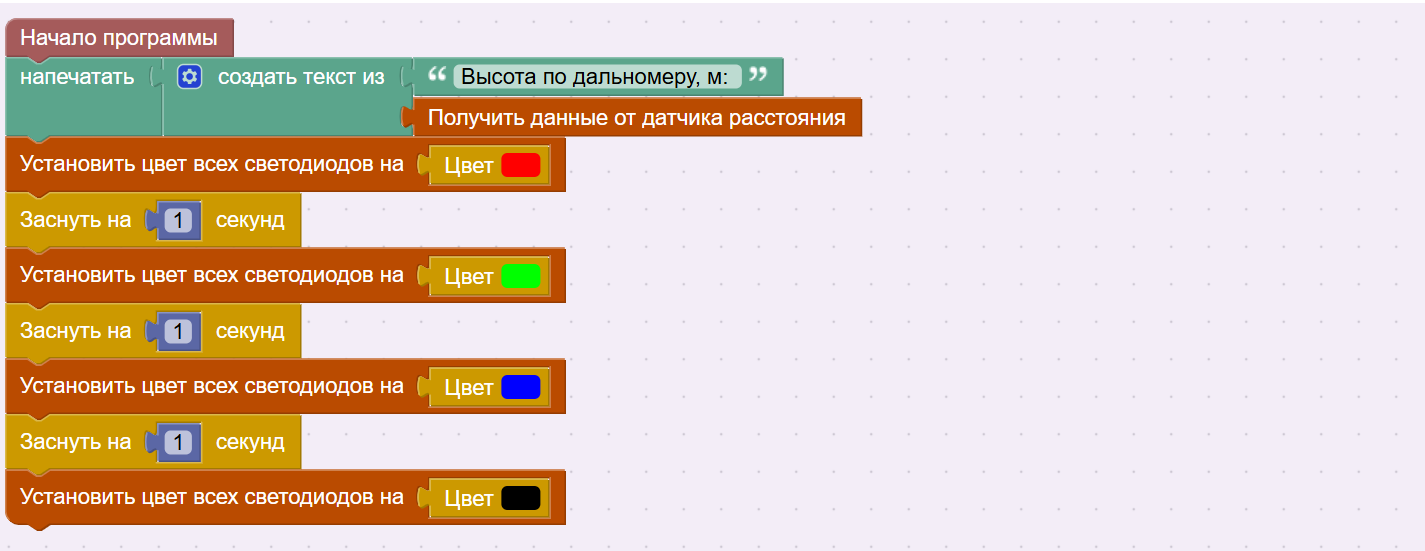
\includegraphics[width=0.62\textwidth]{images/bricks/blocks_u01_svetodiody.png}
\caption{Проект 1: светодиоды красным, зелёным, синим}
\end{figure}

\begin{codefile}[python]{python-onboard/bricks/python/u01_svetodiody.py}
\end{codefile}

\begin{itemize}
  \item Цвет задаётся блоком «Цвет» из категории «Прочее»; Bricks переводит его из вида \texttt{\#RRGGBB} в доли 0..1 для \verb|led_control|. Чёрный цвет --- светодиоды выключены.
  \item «Заснуть на 1 секунд» --- пауза: без неё смена цветов была бы незаметна.
  \item Первый блок «напечатать высоту» нужен из-за особенности Bricks 2.3.0 (раздел~\ref{sec:bricks-limits}): без блока, читающего данные дрона, в программу не попадает строка \verb|pioneer = Pioneer()|.
\end{itemize}

\expected{светодиоды по секунде горят красным, зелёным и синим, затем гаснут.}

\subsubsection*{Проект 2. Бегущий огонь: циклы и переменная-счётчик}

\begin{figure}[H]
\centering
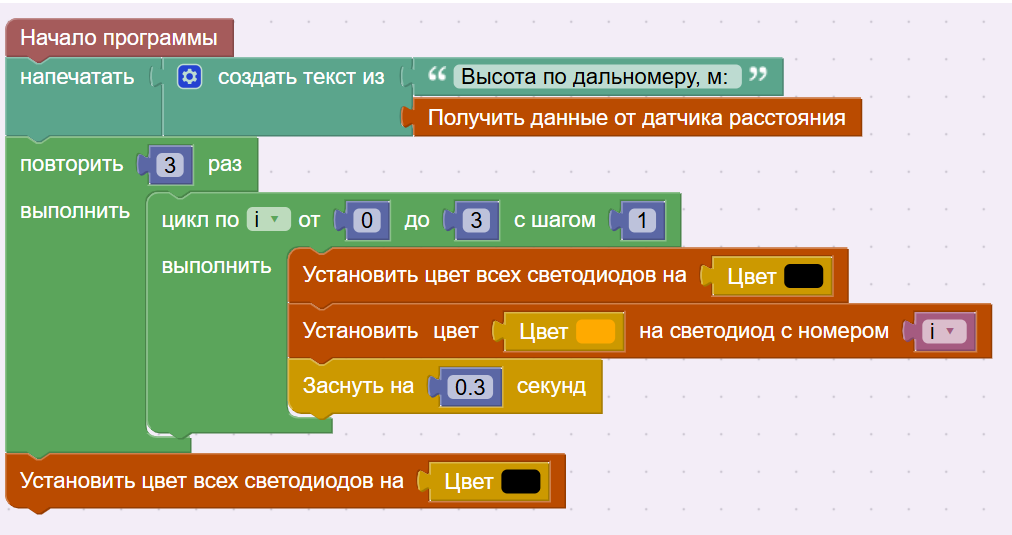
\includegraphics[width=0.72\textwidth]{images/bricks/blocks_u02_beguschiy_ogon.png}
\caption{Проект 2: огонь бежит по четырём светодиодам}
\end{figure}

\begin{codefile}[python]{python-onboard/bricks/python/u02_beguschiy_ogon.py}
\end{codefile}

\begin{itemize}
  \item «повторить 3 раз» --- внешний цикл: огонь пробегает три круга.
  \item «цикл по \texttt{i} от 0 до 3 с шагом 1» --- внутренний цикл; \texttt{i} принимает значения 0, 1, 2, 3 и служит номером светодиода. Bricks превратил его в \verb|range(0, 4)|: граница «до 3» включается.
  \item Перед каждым включением все светодиоды гасятся, поэтому горит ровно один.
\end{itemize}

\begin{taskbox}[Огонь в обратную сторону]
Пустите огонь от 3 до 0 с шагом $-1$. Затем добавьте второй, «догоняющий» огонь другого цвета на светодиоде с номером \texttt{(i + 2) \% 4}.
\expected{по кругу бегут два огонька разных цветов, расстояние между ними не меняется.}
\end{taskbox}

\subsubsection*{Проект 3. Телеметрия: вывод данных}

\begin{figure}[H]
\centering
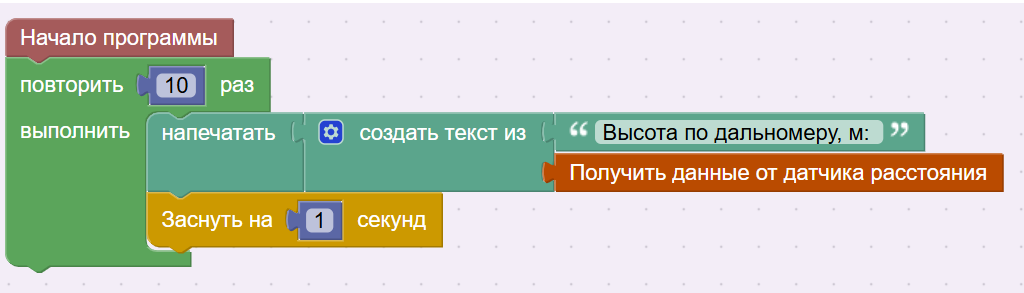
\includegraphics[width=0.75\textwidth]{images/bricks/blocks_u03_telemetriya.png}
\caption{Проект 3: десять измерений высоты}
\end{figure}

\begin{codefile}[python]{python-onboard/bricks/python/u03_telemetriya.py}
\end{codefile}

\begin{itemize}
  \item «создать текст из» склеивает подпись и число; Bricks сам добавил \verb|str(...)|, чтобы склеить строку с числом.
  \item 10 повторений с паузой в секунду --- десять измерений за десять секунд.
\end{itemize}

\expected{в панели «Вывод программы» десять строк «Высота по дальномеру, м: …». Поднимите дрон рукой (при выключенных двигателях!) --- значение изменится.}

\subsubsection*{Проект 4. Светофор высоты: условия}

\begin{figure}[H]
\centering
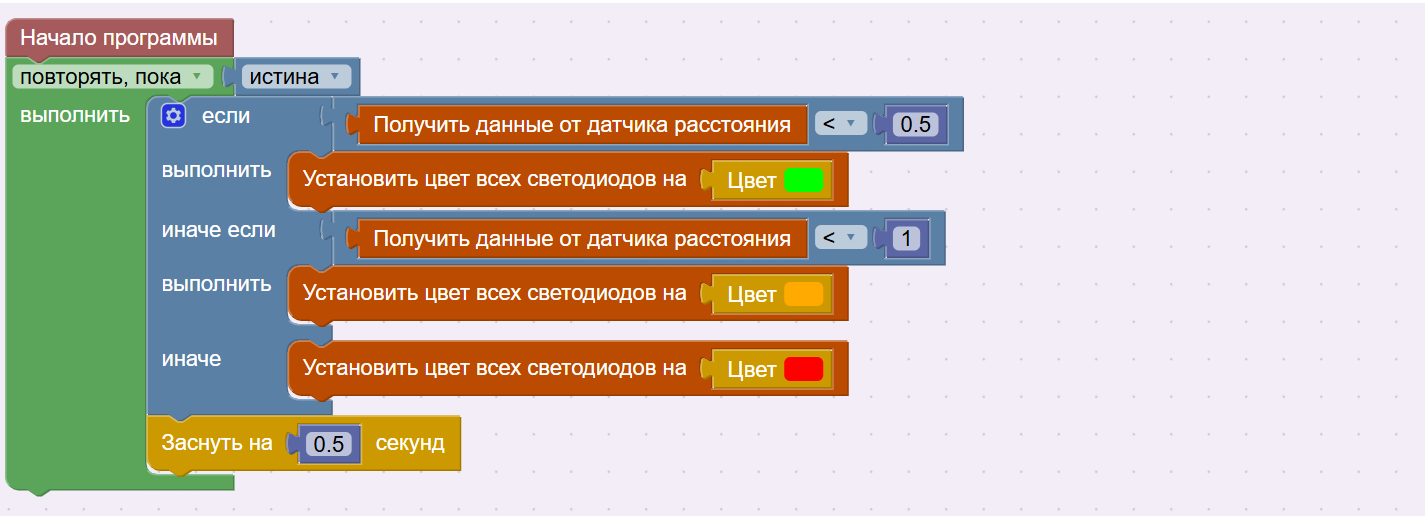
\includegraphics[width=0.72\textwidth]{images/bricks/blocks_u04_svetofor_vysoty.png}
\caption{Проект 4: цвет светодиодов зависит от высоты}
\end{figure}

\begin{codefile}[python]{python-onboard/bricks/python/u04_svetofor_vysoty.py}
\end{codefile}

\begin{itemize}
  \item Ветки проверяются по порядку: ниже 0.5~м --- зелёный; иначе ниже 1~м --- жёлтый; во всех остальных случаях --- красный.
  \item Шестерёнка на блоке «если» добавляет ветки «иначе если» и «иначе».
  \item «повторять, пока истина» --- бесконечный цикл; программа работает до нажатия \ui{Стоп}. Здесь сказывается безопасное завершение: после остановки выполнится \verb|finally|.
\end{itemize}

\begin{taskbox}[Свой светофор]
Добавьте четвёртый уровень: выше 2~м светодиоды мигают красным. Подсказка: понадобится ещё одна ветка «иначе если» и пауза внутри неё.
\expected{при подъёме дрона рукой цвет последовательно меняется зелёный, жёлтый, красный, мигающий красный.}
\end{taskbox}

\subsubsection*{Проект 5. Полёт по квадрату}

\begin{alertbox}[Этот проект поднимает дрон в воздух]
Запускайте его только на подготовленной площадке $2\times2$~м с пультом в руках. При подготовке главы эта программа на дроне \textbf{не запускалась}: показаны только блоки и сгенерированный код. Запускайте сначала с одним отрезком пути.
\end{alertbox}

\begin{figure}[H]
\centering
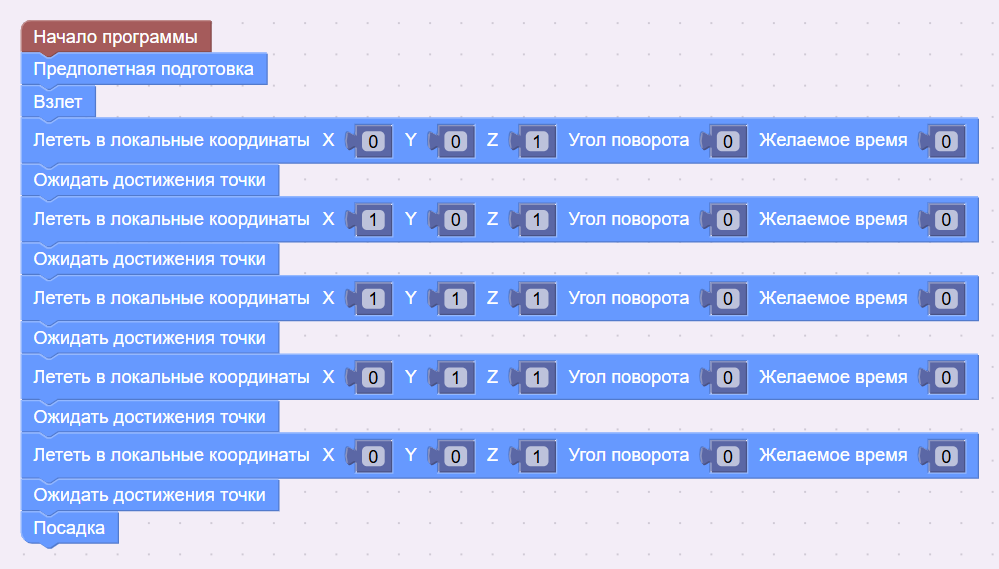
\includegraphics[width=0.85\textwidth]{images/bricks/blocks_u05_polet_kvadrat.png}
\caption{Проект 5: взлёт, четыре точки квадрата, посадка}
\end{figure}

\begin{codefile}[python]{python-onboard/bricks/python/u05_polet_kvadrat.py}
\end{codefile}

\begin{itemize}
  \item «Лететь в локальные координаты» \emph{не ждёт} прилёта, поэтому после каждого полёта стоит «Ожидать достижения точки». Без него дрон сразу получит следующую команду и «срежет» угол квадрата.
  \item Это та же программа, что полёт по квадрату в главе~\ref{sec:sdk2}, только собранная из блоков.
\end{itemize}

\subsubsection*{Проект 6. Фото под разными углами камеры}

\begin{figure}[H]
\centering
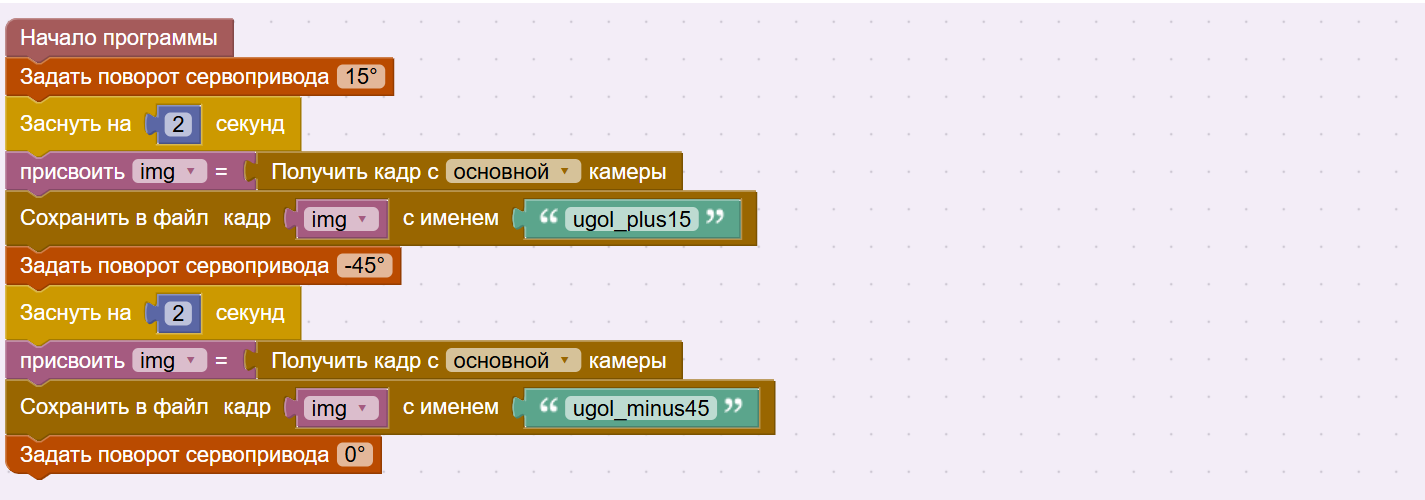
\includegraphics[width=0.6\textwidth]{images/bricks/blocks_u06_foto_ugly.png}
\caption{Проект 6: наклон камеры, кадр, сохранение}
\end{figure}

\begin{codefile}[python]{python-onboard/bricks/python/u06_foto_ugly.py}
\end{codefile}

\begin{itemize}
  \item «Задать поворот сервопривода» --- угол выбирается на циферблате с шагом $15^\circ$ в диапазоне от $-80^\circ$ до $+30^\circ$. Если вписать 20, Bricks округлит до 15 (раздел~\ref{sec:bricks-limits}).
  \item «Сохранить в файл кадр с именем» пишет снимок в \texttt{/mnt/media/photos/<имя>.jpg}: фото сразу видны в «Галерее медиа» Pioneer Code.
  \item Пауза в 2~секунды после поворота нужна, чтобы камера успела повернуться и снимок не смазался.
\end{itemize}

\begin{taskbox}[Фото-серия]
Снимите четыре кадра с углами $0^\circ$, $-30^\circ$, $-60^\circ$, $-75^\circ$ и именами, по которым видно угол. Используйте цикл с переменной или четыре повтора.
\expected{в галерее четыре фото с понятными именами; при большем наклоне в кадре больше пола.}
\end{taskbox}

\subsubsection*{Нейросети и компьютерное зрение}

Блоки ИИ работают так же, как классы \verb|Yolo|, \verb|YoloPose| и \verb|PaddleOCR| из главы~\ref{sec:rknn}: сначала блок «Инициализация ИИ модели» загружает модель на NPU, затем в цикле кадр камеры передаётся модели. Результат удобно смотреть в окне: блок «Демонстрация изображения из кадра … в окно \emph{имя}» публикует кадр, окно открывается по адресу \texttt{http://10.42.0.1:8889/<имя>/}. Проекты 7--10 проверены запуском сгенерированного кода на дроне.

\subsubsection*{Проект 7. Найти людей}

\begin{figure}[H]
\centering
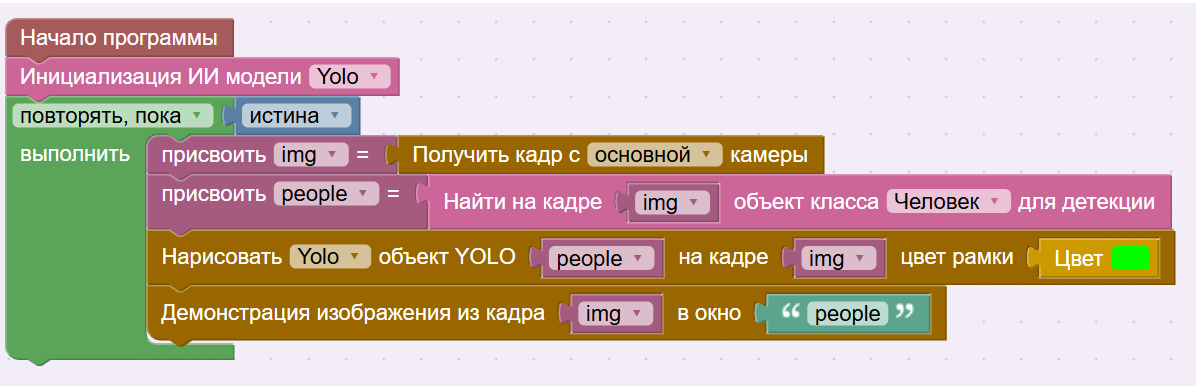
\includegraphics[width=0.95\textwidth]{images/bricks/blocks_u07_ii_lyudi.png}
\caption{Проект 7: детекция людей и рамки на кадре}
\end{figure}

\begin{codefile}[python]{python-onboard/bricks/python/u07_ii_lyudi.py}
\end{codefile}

\begin{itemize}
  \item «Найти на кадре \texttt{img} объект класса Человек» --- детекция с фильтром по классу (в списке 80 классов COCO по-русски). Результат сохраняется в переменную \texttt{people}.
  \item «Нарисовать Yolo объект \texttt{people} на кадре \texttt{img}» рисует рамки, «Демонстрация…» отправляет кадр в окно \texttt{people}.
  \item Bricks сам добавил кэш \verb|infer_cache_per_frame|: если на одном кадре нейросеть вызывается несколько раз, она считает его один раз.
\end{itemize}

\begin{figure}[H]
\centering
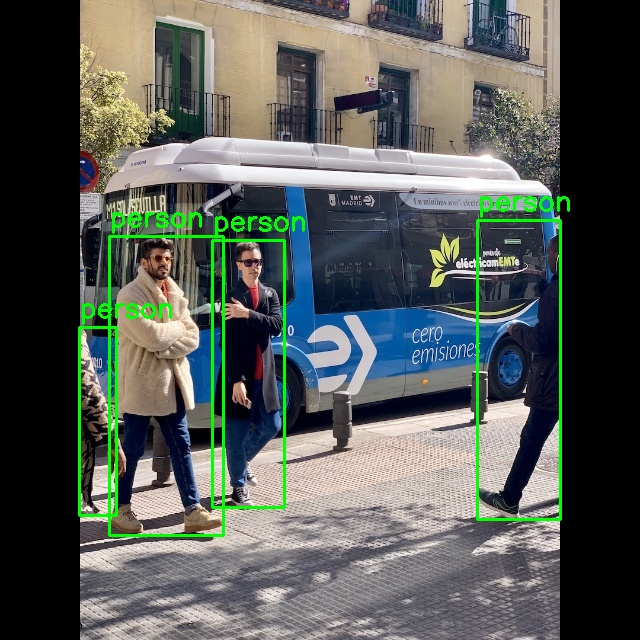
\includegraphics[width=0.45\textwidth]{images/bricks/br07_people_2.jpg}
\caption{Результат проекта 7 на дроне (на вход подано тестовое изображение): рамки вокруг людей, автобус не выделен --- работает фильтр «Человек»}\label{fig:bricks-people}
\end{figure}

\expected{окно \texttt{http://10.42.0.1:8889/people/} с рамками вокруг людей; на дроне программа обрабатывала около 7--8 кадров в секунду.}

\subsubsection*{Проект 8. Жест «две руки вверх» включает свет}

\begin{figure}[H]
\centering
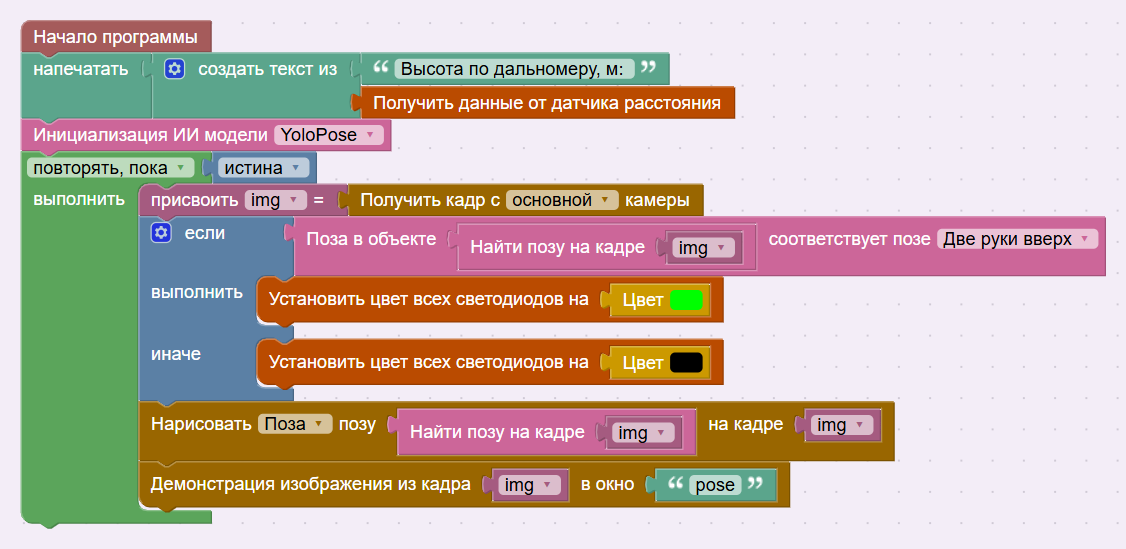
\includegraphics[width=0.9\textwidth]{images/bricks/blocks_u08_ii_zhest.png}
\caption{Проект 8: поза человека управляет светодиодами}
\end{figure}

\begin{codefile}[python]{python-onboard/bricks/python/u08_ii_zhest.py}
\end{codefile}

\begin{itemize}
  \item «Поза в объекте … соответствует позе Две руки вверх» возвращает «истину», только если жест держится несколько кадров подряд (параметр \verb|THRESHOLD| в сгенерированном коде). Это защита от случайных срабатываний: тот же приём устойчивого решения по нескольким кадрам вы встретили в главе~\ref{sec:rknn}.
  \item Доступные позы: левая и правая рука вверх или в сторону, две руки вверх, обе в стороны, кисти рядом в центре.
  \item «Нарисовать Позу» рисует скелет на кадре, окно называется \texttt{pose}.
\end{itemize}

\expected{поднимите обе руки --- через несколько кадров светодиоды загорятся зелёным; опустите --- погаснут.}

\subsubsection*{Проект 9. Распознать текст}

\begin{figure}[H]
\centering
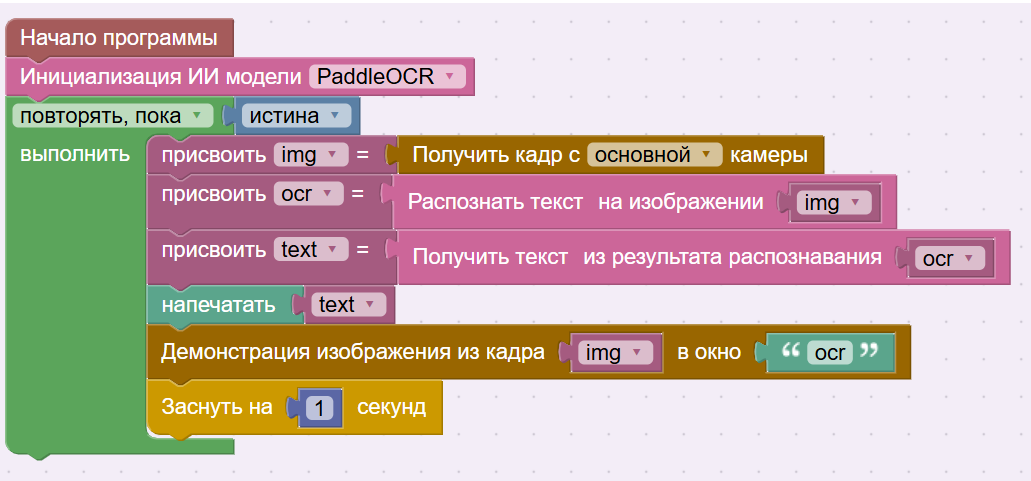
\includegraphics[width=0.78\textwidth]{images/bricks/blocks_u09_ii_tekst.png}
\caption{Проект 9: распознавание текста PaddleOCR}
\end{figure}

\begin{codefile}[python]{python-onboard/bricks/python/u09_ii_tekst.py}
\end{codefile}

\begin{itemize}
  \item Результат распознавания сначала сохраняется в переменную \texttt{ocr}, и только потом из него извлекается текст. Если вложить блоки друг в друга напрямую, Bricks~2.3.0 сгенерирует код с синтаксической ошибкой (раздел~\ref{sec:bricks-limits}).
  \item «Заснуть на 1 секунд»: распознавание тяжёлое, чаще раза в секунду оно обычно и не нужно.
\end{itemize}

\begin{figure}[H]
\centering
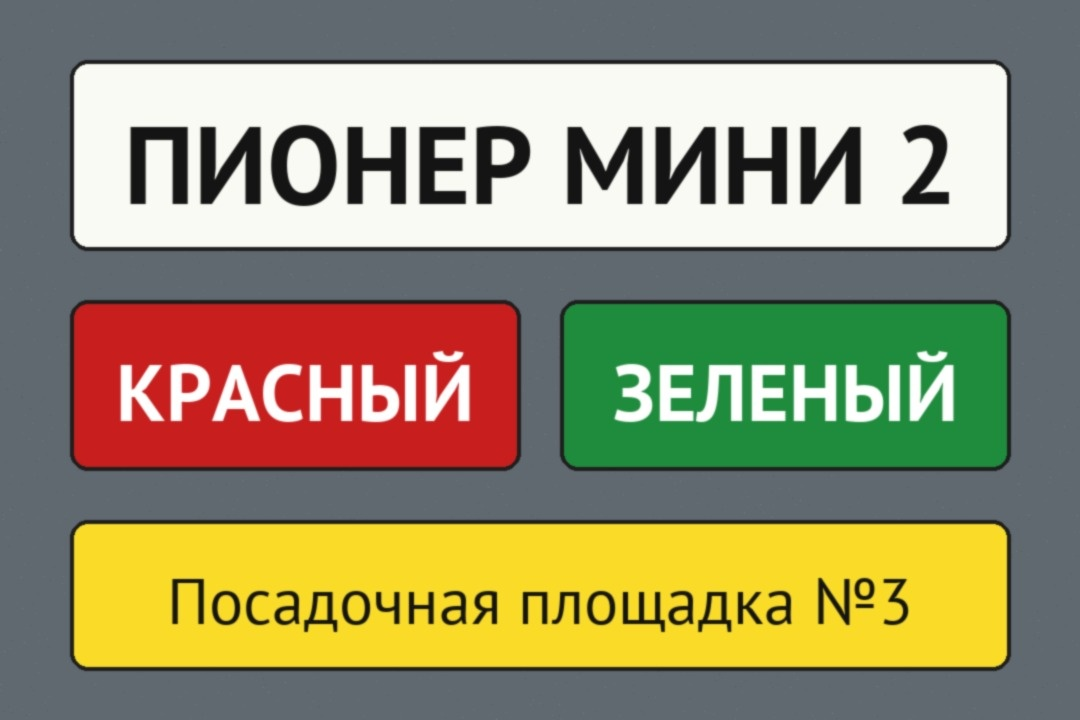
\includegraphics[width=0.6\textwidth]{images/bricks/br09_ocr_2.jpg}
\caption{Окно \texttt{ocr} программы на дроне (на вход подана табличка с текстом)}\label{fig:bricks-ocr}
\end{figure}

Вывод программы на дроне для таблички с рис.~\ref{fig:bricks-ocr}:

\begin{verbatim}
ПИОНЕР МИНИ2
КРАCНЬИ
зеленый
Посадочная площадка
\end{verbatim}

В слове «КРАCНЬИ» вторая буква~С латинская: модель смешивает похожие буквы двух алфавитов, поэтому результат сравнивают по смыслу, а не посимвольно.

\begin{infobox}[Окно ocr появляется не сразу]
Распознавание медленное, да ещё в цикле стоит пауза в секунду: в окно уходит меньше одного кадра в секунду. Поэтому окно \texttt{http://10.42.0.1:8889/ocr/} начинает показывать видео только через 20--30 секунд после запуска --- браузер ждёт первого полного (ключевого) кадра. Уберите блок «Заснуть», если нужно более живое изображение.
\end{infobox}

\subsubsection*{Проект 10. Маркеры ArUco}

\begin{figure}[H]
\centering
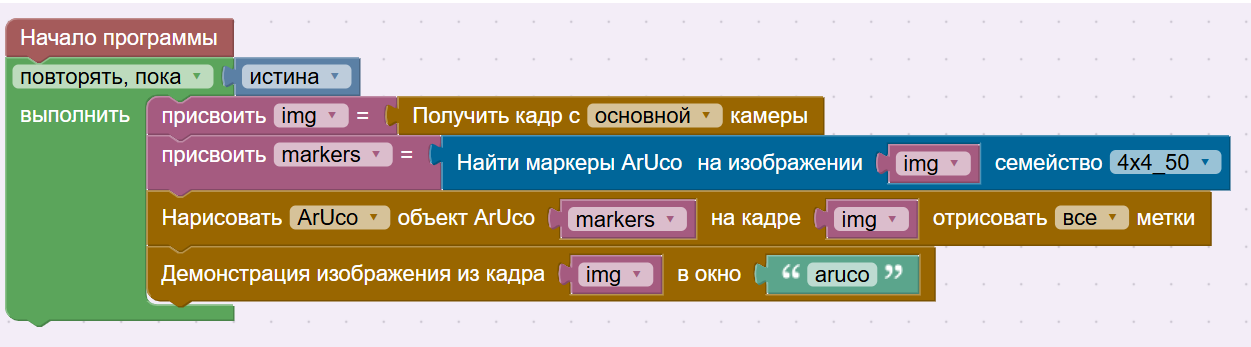
\includegraphics[width=0.95\textwidth]{images/bricks/blocks_u10_aruco.png}
\caption{Проект 10: поиск и отрисовка маркеров ArUco}
\end{figure}

\begin{codefile}[python]{python-onboard/bricks/python/u10_aruco.py}
\end{codefile}

\begin{itemize}
  \item «Найти маркеры ArUco на изображении \texttt{img} семейство 4x4\_50» --- семейство должно совпадать с напечатанными маркерами.
  \item Блоки «Координаты объекта» и «Размер объекта» из «Компьютерного зрения» дают центр и размер маркера с нужным ID --- с ними можно, например, поворачивать дрон к маркеру.
\end{itemize}

\expected{в окне \texttt{http://10.42.0.1:8889/aruco/} найденные маркеры обведены и подписаны номерами; на дроне программа работала с частотой около 7 кадров в секунду.}

\begin{taskbox}[Маркер в центре]
Выведите в «Вывод программы» координаты центра маркера с ID~0. Включайте зелёный свет, когда маркер находится в центральной трети кадра, и красный --- когда нет.
\expected{при смещении маркера в кадре цвет светодиодов меняется на границах центральной трети; координаты в выводе согласованы с положением маркера.}
\end{taskbox}

\subsection{Особенности и ограничения Bricks 2.3.0}\label{sec:bricks-limits}

Сгенерированный код каждого проекта проверяли. Вот что обнаружено.

\begin{center}\small
\begin{tabularx}{\linewidth}{@{}>{\raggedright\arraybackslash}p{0.3\linewidth}X@{}}
\toprule
\textbf{Ситуация} & \textbf{Что происходит и как обойти} \\
\midrule
Программа только из блоков светодиодов &
  блок светодиодов не добавляет в код \verb|pioneer = Pioneer()|; программа завершится с ошибкой \verb|name 'pioneer' is not defined|. \textbf{Обход:} поставьте в начало любой блок, читающий данные дрона (например, «напечатать» и «Получить данные от датчика расстояния») --- проекты 1, 2, 8 \\
«Распознать текст» вставлен прямо в «Получить текст из результата…» &
  генерируется \verb|:=| внутри генератора списка --- \verb|SyntaxError| в Python 3.12, программа не запускается. \textbf{Обход:} сохраните результат в переменную (проект 9) \\
Угол сервопривода &
  поле-циферблат округляет угол до шага $15^\circ$: 20 превращается в 15, $-40$ в $-45$ \\
Длинные блоки &
  вложенные блоки быстро становятся очень широкими; удобнее сохранять промежуточные результаты в переменные (проекты 7, 9, 10) \\
\bottomrule
\end{tabularx}
\end{center}

\begin{infobox}[Версия 2.3.0]
Список относится к Bricks~2.3.0 на Pioneer~OS 1.0.0; в других версиях поведение может отличаться. Если сомневаетесь, откройте сгенерированный \texttt{.py} и сравните с таблицей соответствия блоков.
\end{infobox}

\subsection{Блоки и Python: что с чем сравнивать}

Каждый из десяти проектов можно написать на Python из глав~\ref{sec:sdk2} и~\ref{sec:rknn}; это хороший способ закрепить и то, и другое.

\begin{center}\small
\begin{tabularx}{\linewidth}{@{}>{\raggedright\arraybackslash}p{0.38\linewidth}X@{}}
\toprule
\textbf{Проект Bricks} & \textbf{Где то же на Python} \\
\midrule
1, 2 --- светодиоды, циклы & светодиоды в главе~\ref{sec:sdk2} \\
3, 4 --- телеметрия, условия & дальномер и датчики в главе~\ref{sec:sdk2} \\
5 --- полёт по квадрату & полёт по точкам в главе~\ref{sec:sdk2} \\
6 --- сервопривод и фото & камера и сервопривод в главе~\ref{sec:sdk2} \\
7 --- найти людей & детекция \verb|Yolo| в главе~\ref{sec:rknn} \\
8 --- жесты & \verb|YoloPose| в главе~\ref{sec:rknn} \\
9 --- текст & \verb|PaddleOCR| в главе~\ref{sec:rknn} \\
10 --- ArUco & маркеры ArUco в главе~\ref{sec:python-vision}, с учётом кадра из \verb|Camera| \\
\bottomrule
\end{tabularx}
\end{center}

\begin{taskbox}[Из блоков в Python]
Выберите любой из проектов 1--4, откройте его сгенерированный \texttt{.py} и перепишите тело программы на Python вручную: без \verb|hex_to_bgr|, с обычными числами для цвета. Запустите в Pioneer Code.
\expected{ваша программа делает то же, что и блочная: те же цвета, паузы и вывод; \texttt{finally} с посадкой у вас на месте.}
\end{taskbox}

\begin{taskbox}[Свой проект]
Соберите в Bricks программу, которая показывает на светодиодах расстояние до препятствия: дальномер Ranger или датчик высоты, три цвета и пауза в полсекунды. Сохраните проект, экспортируйте его в \texttt{.xml} и импортируйте на соседний дрон.
\expected{цвет светодиодов меняется вместе с расстоянием; проект открывается на другом дроне без правок.}
\end{taskbox}

\begin{taskbox}[Где ошибка]
Соберите блок «Распознать текст» прямо внутри «Получить текст из результата…» и сохраните проект. Откройте сгенерированный код, найдите строку с \verb|:=| и исправьте проект через переменную \texttt{ocr}.
\expected{без переменной программа не запускается (\texttt{SyntaxError}), с переменной --- печатает распознанный текст.}
\end{taskbox}

\begin{missionbox}[Миссии симулятора к главе]
Режим \ui{Обучение} содержит трек «\ui{Мини 2 · Bricks}»: 16 миссий на блоках Pioneer Bricks. Миссия открывает дрон Пионер Мини~2 и редактор блоков Bricks, проверяет состав блоков и полёт в симуляторе. Миссии идут по проектам и логике главы: первые блоки и взлёт (1--2), светодиоды (проект~1, миссии 3--4), циклы и бегущий огонь (проект~2, миссии 5--6), данные и условия (проекты 3 и~4, миссии 7--9), полёт по точкам и квадрату (проект~5, миссии 10--12), камера, сервопривод и фото (проект~6, миссии 13--14), метки ArUco (проект~10, миссия 15) и итоговый световой патруль (16). Проекты 7--9 с нейросетями (люди, жесты, текст) и блоки с пометкой «только на дроне» в трек не вошли.
\end{missionbox}

